\chapter{绪论}

\section{课题来源}
红外目标检测是指用红外探测器检测目标与背景之间的红外辐射差异后,对目标进行检测的过程。虽然可见光图像具有图像分辨率高、目标细节完整的特点,但是与红外图像相比容易受到光线变化的影响,大大增加了识别目标的难度。在一些特殊的天气条件下尤其如此,例如下雨天、夜间、有雾天和缺乏可见光源的天气,视距和能见度很低,并且捕获的图像无法正常使用。红外成像技术的特点是工作距离远、抗干扰能力强、测量精度高、受天气影响较小。日夜工作和强大的烟雾穿透能力强使得红外目标检测的市场需求也在不断增加,红外目标检测不仅仅用于军事领域,在工业、安防、交通等民用领域也有广泛的应用,比如红外技术可以应用在无人机上进行全天候的目标检测;在工业界,设备有没有被严重触碰或损坏也可以应用红外技术。尤其是今年疫情期间,红外技术广泛应用于火车站、机场等人流密集的地方,能够实现实时检测体温,避免人工测量体温而造成的拥堵。

本课题主要研究红外图像中的无人机检测算法。本课题来源于哈尔滨海邻科信息技术有限公司“警用人工智能技术合作”。目前,无人机市场发展迅速,为社会带来便利。国外机场无人机干扰航班事件频发,各地无人机“黑航”事件频发。该国军队也受到了部队内外的广泛关注,给机场安全、反恐维稳和国家边境带来了相当大的压力,迫切需要通过对无人机的探测来对无人机施行监控和预警。使用声音、无线电和雷达探测的技术更为常见,但这些技术通常需要昂贵的设备和严格的配置。基于机器视觉的方法具有成本低、配置简单的优点。随着深度学习技术的发展,逐渐应用于各种目标的识别和检测,但是无人机往往在低空飞行,并且还受到光线和遮挡的影响。检测场景非常复杂,而小尺寸和高速度一直是目标检测的难题。相关监管部门应利用相关检测网络及时发现管制区域内的非法无人机,以保障人身安全和财产安全。因此,本课题的目的是研究和设计无人机检测算法,以实现快速高效的红外无人机检测。

\section{研究背景与意义}
计算机视觉技术是一种让计算机从给定的图像或视频中获取相关信息并进行“感知”的技术,是人类视觉感知的扩展。半导体行业促进了硬件水平的提高,也带动了机器视觉的发展,使其在人工智能领域得到广泛应用。

在计算机视觉领域中,基于红外探测系统的红外弱小目标检测一直都是一个重要的课题和研究热点。当前主流的探测系统可分为3类:可见光探测、红外成像探测和雷达探测系统。红外探测系统只对目标的温度与本身的材料特性敏感,而与环境等因素无关,使得其在3类探测系统中脱颖而出,具有一系列优势:
(1)不受光照的影响,可以全天时工作;
(2)由于其不发射电磁波,因此是非自动的探测方法;
(3)穿透能力强,可以避免灰尘、云层和烟雾等的遮挡,可以更好地识别虚假的伪装目标。以上优势也使其成为传统可见光探测系统与雷达探测系统的有效补充或替代。

随着各方面技术的成熟,研究人员在不断提高红外探测系统的性能。红外探测技术广泛应用于军事领域,如红外预警、水下搜索和红外导航中,还应用于医疗损伤、细胞诊断、工业探伤等民用领域。在军事和包括医疗在内的民用领域取得突出成就。实时检测红外目标,高检出率、低误报率是实际应用中重要的要求。一般情况下,待检测目标与检测器之间的距离较长,因此,红外目标在整个红外图像中占据的区域非常小。它们通常小于 100 像素,背景复杂、易变且难以检测。具体表现如下:

(1)红外目标的特点:弱小红外目标缺乏颜色、纹理等属性,尺寸较小。 (通常小于 9×9 像素)大多数方法仅适用于灰度分布特征、运动属性和运动方向等特征。此外,小型红外目标的信噪比较低。并且经常被复杂而动态的背景所掩盖,还会受到云层和海浪的干扰。

(2) 红外背景的特点:背景相似,分布连续。目标通常在云和波浪中。场景复杂多变。复杂红外图像的背景特征有些不均匀,并且相对灰度比目标区域低。

(3) 红外目标检测困难: 1) 目标可用特征较少。因为目标很小,所以总辐射能量小于背景辐射能量。图像中的灰度分布是可变的,很难使用统一的数学模型来描述,而且它缺乏传统可见光目标的纹理、形状和其他结构信息。传统可见光检测方法不能用于检测小而弱的红外目标,或是一般性能较差。 2)图像信噪比低。由于成像距离远,小目标难以和杂波和噪声区分开,容易被淹没在云层和海浪中,使得检测算法容易受到干扰。 3)检测精度不高。在实际情况和使用中,目标的运动方向和速度具有很强的机动性。这使得提高机动目标的检测精度成为学术界致力于解决的问题。4)成像环境复杂。在精确的红外制导和预警方面,成像过程往往伴随着烟雾和海浪。这导致对不同检测算法的鲁棒性提出更高的要求。 5)实时性差。检测效果通常与计算量成近似反比。检测效果好的算法往往需要大量的计算。因为建模体积大、硬件处理能力不足,常常导致实时性能不佳。6)很少有公开数据集。红外目标检测主要用于军事领域,具有一定的保密性。可供研究人员公开使用的红外数据集很少,这在一定程度上限制了红外目标检测算法的发展。本课题检测的目标图像如图\ref{uav}所示。

\begin{figure}[htbp]
    \centering
    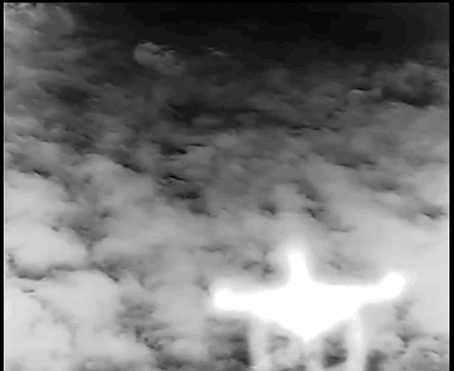
\includegraphics[width = 0.8\textwidth]{无人机目标示例.png}
    \caption{无人机目标示意图}
    \label{uav}
\end{figure}

综上所述,红外图像的目标检测应用广泛,具有很大的研究价值。本文基于深度学习算法,针对红外无人机目标进行研究,针对红外图像无人机目标检测的特点,从数据增强、网络结构改进、网络轻量化、嵌入式实现这四个方面展开研究。

\section{国内外研究发展现状}
目标检测包括目标分类和目标定位两个子任务,用于检测视频中特定类别的语义对象实例。本文从传统的目标检测、基于深度学习的two-stage目标检测算法、基于深度学习的one-stage目标检测算法三个阶段介绍目标检测算法的发展过程\cite{尹宏鹏2016基于视觉的目标检测与跟踪综述}。

\subsection{传统的目标检测算法}
如图\ref{ct}所示,传统的目标检测算法流程是先选定目标区域,经过特征提取之后通过分类器分类得到检测结果。

\begin{figure}[htbp]
    \centering
    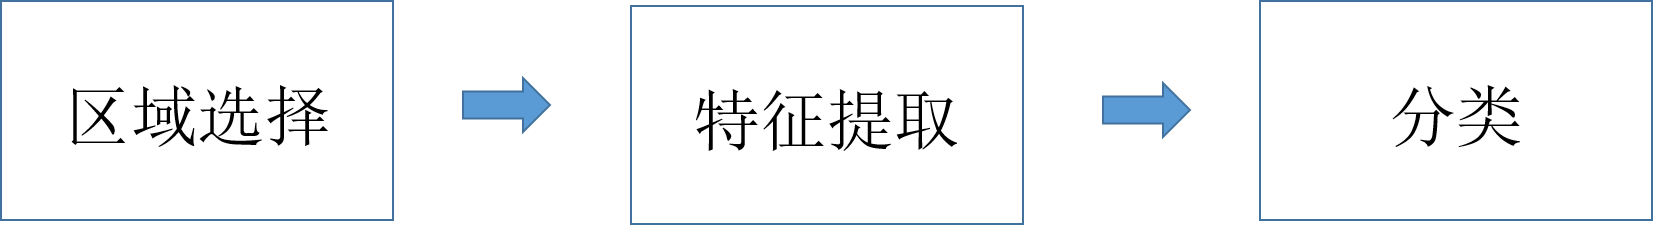
\includegraphics[width = 0.9\textwidth]{传统目标检测.png}
    \caption{传统目标检测流程}
    \label{ct}
\end{figure}

在传统的目标检测算法中,最初区域选择采用不同尺度长宽比的滑动窗口遍历整幅图像,框出候选区域即可能包含目标的区域\cite{胡伏原2020基于卷积神经网络的目标检测算法综述,kira1992feature}。这种穷举的方法时间复杂度高,会产生大量冗余窗口,会影响之后的特征提取及分类的速度和精度。后来发展出更加高效的区域选择算法,如Selective Search\cite{uijlings2013selective},  Edge Boxes\cite{zitnick2014edge}等。Selective Search将图片划分成很多的小区域,然后根据计算得到的两两区域之间的相似度及区域的大小不断地聚合相邻的小区域,重复上述过程直到整张图片组合成一个大的区域。Edge Boxes利用edge group之间的相似性,根据权值判断box中包含的轮廓数或与box边界重叠的轮廓数,基于以上信息对box进行打分,然后根据box得分的高低顺序确定候选区域的信息。第二步从候选区域提取固定长度的特征向量,来获取此区域的判别语义信息。传统的机器学习采用手工特征作为机器学习模型的输入,目标检测领域也是如此。但是由于目标的形态多种多样,光照变化及背景的多样性等因素使得设计一种鲁棒的特征不是很容易,并且提取到的特征好坏直接影响到之后分类的准确性。在这一阶段,常用的图像特征有HOG特征\cite{he1990texture}和SIFT特征\cite{lowe1999object}等。HOG将图像分割成一个个小的连通区域(细胞单元),在每个单元内部采集每个像素点的梯度或边缘的梯度直方图,得到的直方图就是这个单元的特征。SIFT特征提取算法首先对输入的图像在DoG尺度空间上提取极值点,然后对尺度空间DoG函数进行拟合,进行关键点的精确定位,去除不稳定的关键点。然后计算剩余的关键点的主方向,构造SIFT描述子。SIFT特征由于其具有尺度、旋转不变性,并且能够适应复杂的光照变化,因此常用于传统的目标检测领域。第三步提取特征之后,用分类器进行分类,分类算法有Adaboost算法\cite{freund1997decision}和SVM分类器\cite{cortes1995support}。

传统的目标检测算法主要存在以下两个问题:一是计算的复杂度高,区域选择策略没有针对性,具有窗口冗余,会导致后续分类过程出现错检的现象;二是手工设计的特征对于环境多样性没有很好的鲁棒性,对于复杂环境情况下手工设计的特征没有办法获取准确的语义信息,检测的精度不高。相对于传统的目标检测算法,深度卷积神经网络能够从训练数据的过程中自动的获取图像中的层次特征表示,如低层次的卷积获取位置信息,高层次的卷积获取目标语义信息。同时如果使用的数据集越大学习到的信息更多,表示能力越强。因此在卷积神经网络提出后,基于卷积神经网络的目标检测算法快速发展,相比于传统算法表现出很多优势。

\subsection{基于深度学习的two-stage目标检测算法}
two-stage目标检测算法也称为基于候选框的目标检测算法。这种目标检测算法主要分两步进行:

(1)先在输入图像中选出候选区域。常用的算法有Selective Search和Edge Boxes。

(2)在候选区域上使用CNN网络进行提取特征和分类。

2014年,2014 年,Girshick 等人开创性地提出使用 Selective Search+CNN 代替传统的
滑动窗口+手工特征提出了 R-CNN 模型框架\cite{girshick2014rich},证明了 CNN 相比于传统的 HOG
等手工特征在 PASCAL VOC 2007 上目标检测性能提升的更显著,深度学习算法
在目标检测领域是有效和高效的,开启了基于深度学习的目标检测热潮。如图
\ref{rcnn}所示,R-CNN 由 4 个独立的步骤组成:

\begin{figure}[htbp]
    \centering
    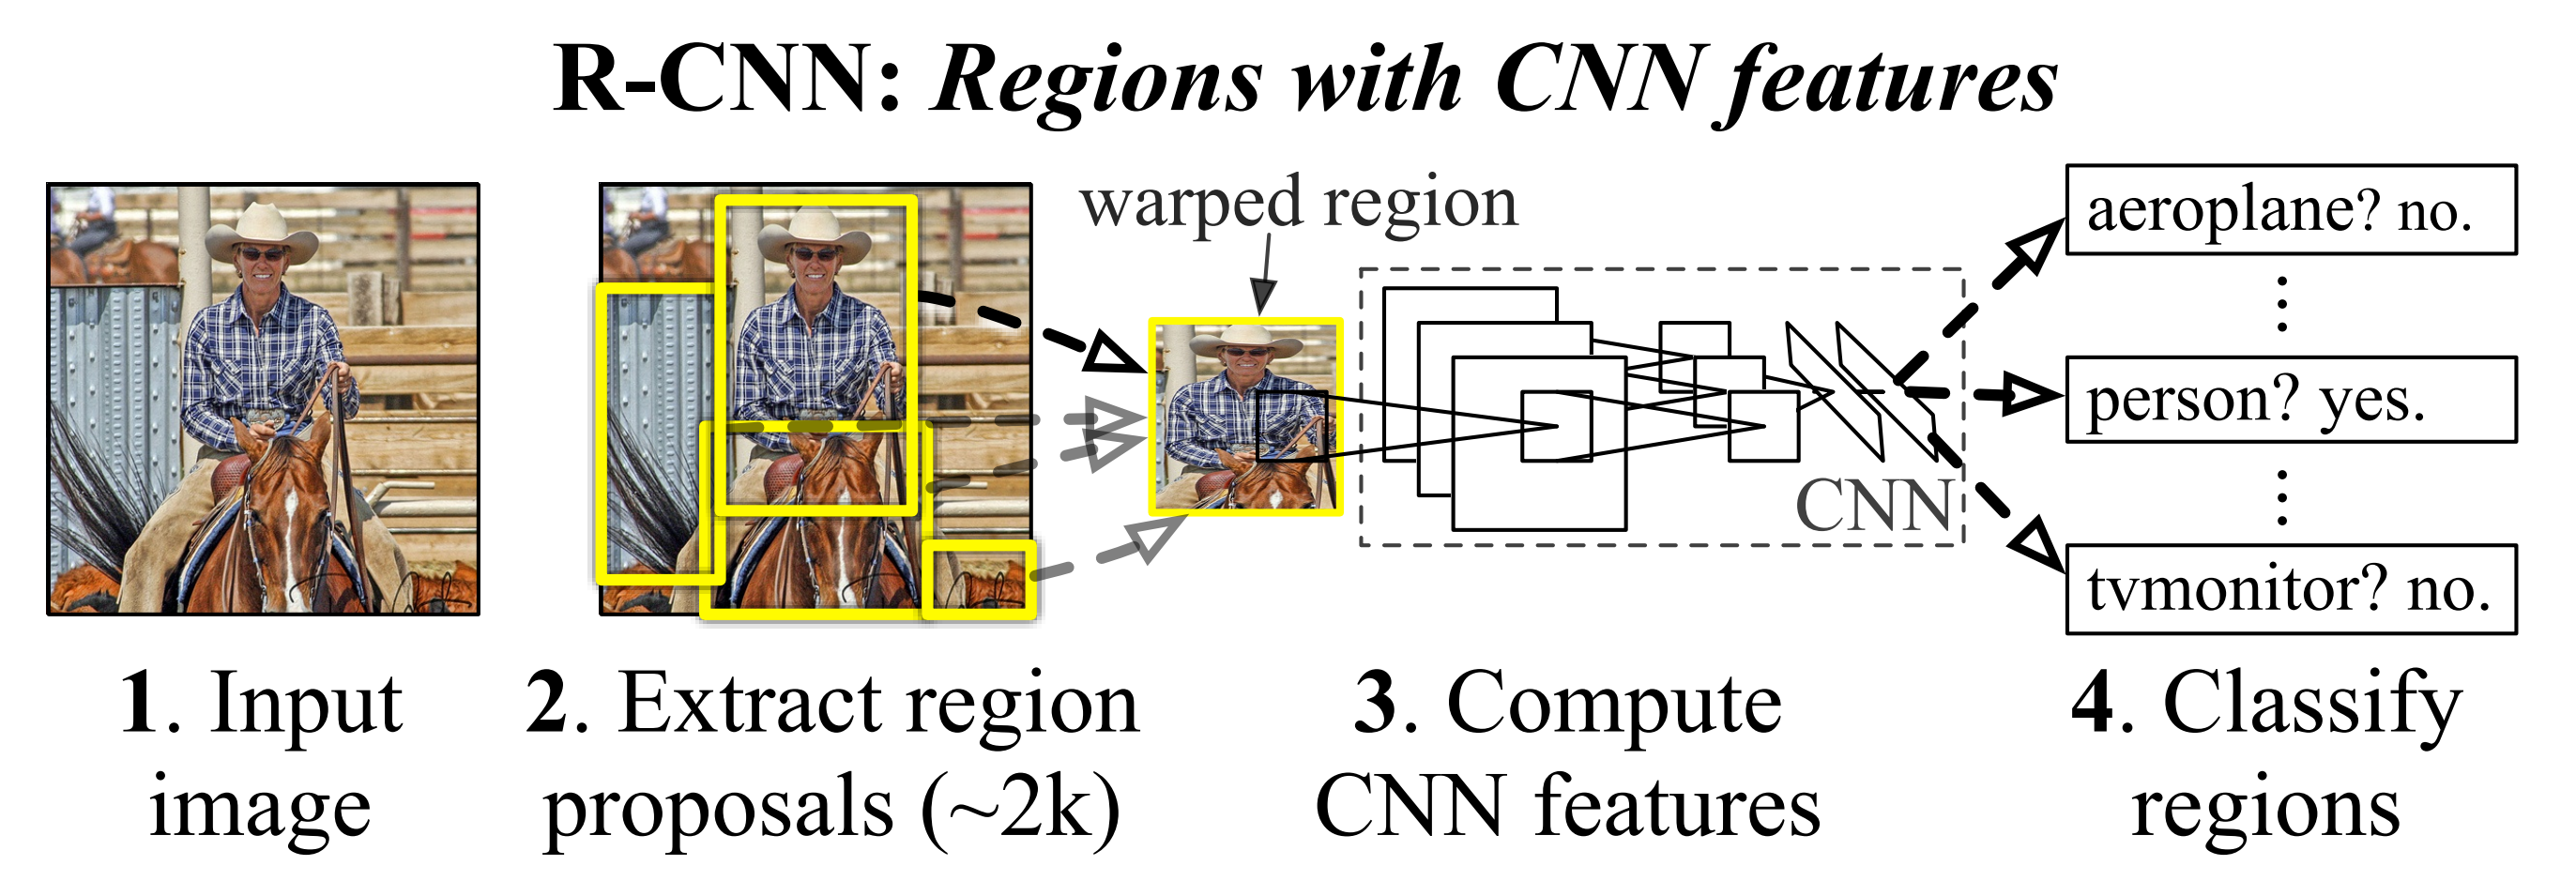
\includegraphics[width = 0.9\textwidth]{rcnn.png}
    \caption{R-CNN算法框架}
    \label{rcnn}
\end{figure}

(1)对于每张图片使用 Selective Search
算法产生 1K~2K 候选区域,并把这些区域调整到固定大小(因为全连接层需要
输入固定长度的矢量)。

(2)对每个候选区域使用 CNN 提取特征输出为特征向
量。

(3)把提取到的特征向量用 SVM 分类器分类,每个类别拥有训练好的分
类器,分类器之间参数不共享。

(4)使用 bounding-box 回归器对候选框位置修
正。相比于传统的目标检测算法,CNN 能够在不同层网络捕捉到不同的目标尺
寸信息,最终生成能够充分表征目标特征的 feature map。该模型使用 AlexNet 网
络结构借鉴 fine-tuning 思想,在 PASCAL VOC 2007 数据集上的准确率达到 58%,使用 VGG16 网络结构在 PASCAL VOC 2007 数据集上的准确率达到 66%,相比
传统算法高了约 20%。
但是 R-CNN 也存在着以下问题:

(1)整个网络结构训练分为好几个阶段,
步骤繁琐。

(2)每张图片提取到的候选区域过多,存在冗余,训练耗时并且在
复杂场景下使用 Selective Search 算法很难提取到高质量的候选框。

(3)提取到的候选框是分别进入到 CNN 网络中进行特征提取,导致大量的重复计算,速度
慢。

之后何凯明等人受到空间金字塔匹配(SPM)概念的启发,针对 R-CNN 在
提取特征时存在重复计算问题提出了 SPP-Net\cite{purkait2017spp},改善了 R-CNN 对所有的候选
区域需要分别输入网络提取特征的缺点,一次性对整张图片利用 CNN 提取特征
并通过 SPP 将提取到的特征转变成固定长度的特征向量输入到全连接层,加速
了 R-CNN 的推理速度,减少了计算量。SPP 是不经过 R-CNN 原来将候选区域
调整到固定输入大小的处理步骤,因此不会存在信息的丢失和几何失真。但
SPP-Net 的局限就是不能使用梯度反传(BP),导致某些层的参数没有办法更新
并且训练仍然是多阶段的。针对 SPP-Net 存在的两个局限,2015 年 Girshick 提
出的 Fast R-CNN\cite{girshick2015fast}融合了 SPP-Net 和 R-CNN 的优点,将整张图像一次性输入网
络中进行提取特征,并引用多任务损失函数(分类和回归)使得整个训练过程除
了候选区域提取阶段以外的过程实现端到端优化,弥补了 R-CNN 多阶段训练及
存储消耗的时间和资源。主要的创新点在于:

(1)将分类损失和回归损失放到
一起进行网络的训练并用 softmax 替原来的 SVM 分类器。

(2)ROI pooling。ROI
pooling layer 是相比于 SPP-Net 空间金字塔池化层的简洁版,主要作用为将图像
在输入网络之前计算得到的候选框映射到最后一个卷积层输出的 feature map 上,
经过 ROI pooling 输出固定大小(一般所使用的为 max pooling)。整个算法在
PASCAL VOC 2007 数据集上 mAP 达到 66.9%,相比于 R-CNN 虽然才涨了 0.9
个点,但是训练速度却是 R-CNN 的 9 倍。该算法的局限性在于 Selective Search
或 Edge Boxes 算法是基于低级视觉信息,无法以数据驱动的方式进行学习,并
且提取候选框过程在目标检测中耗时过多。算法框架如图\ref{fastr}所示。

\begin{figure}[htbp]
    \centering
    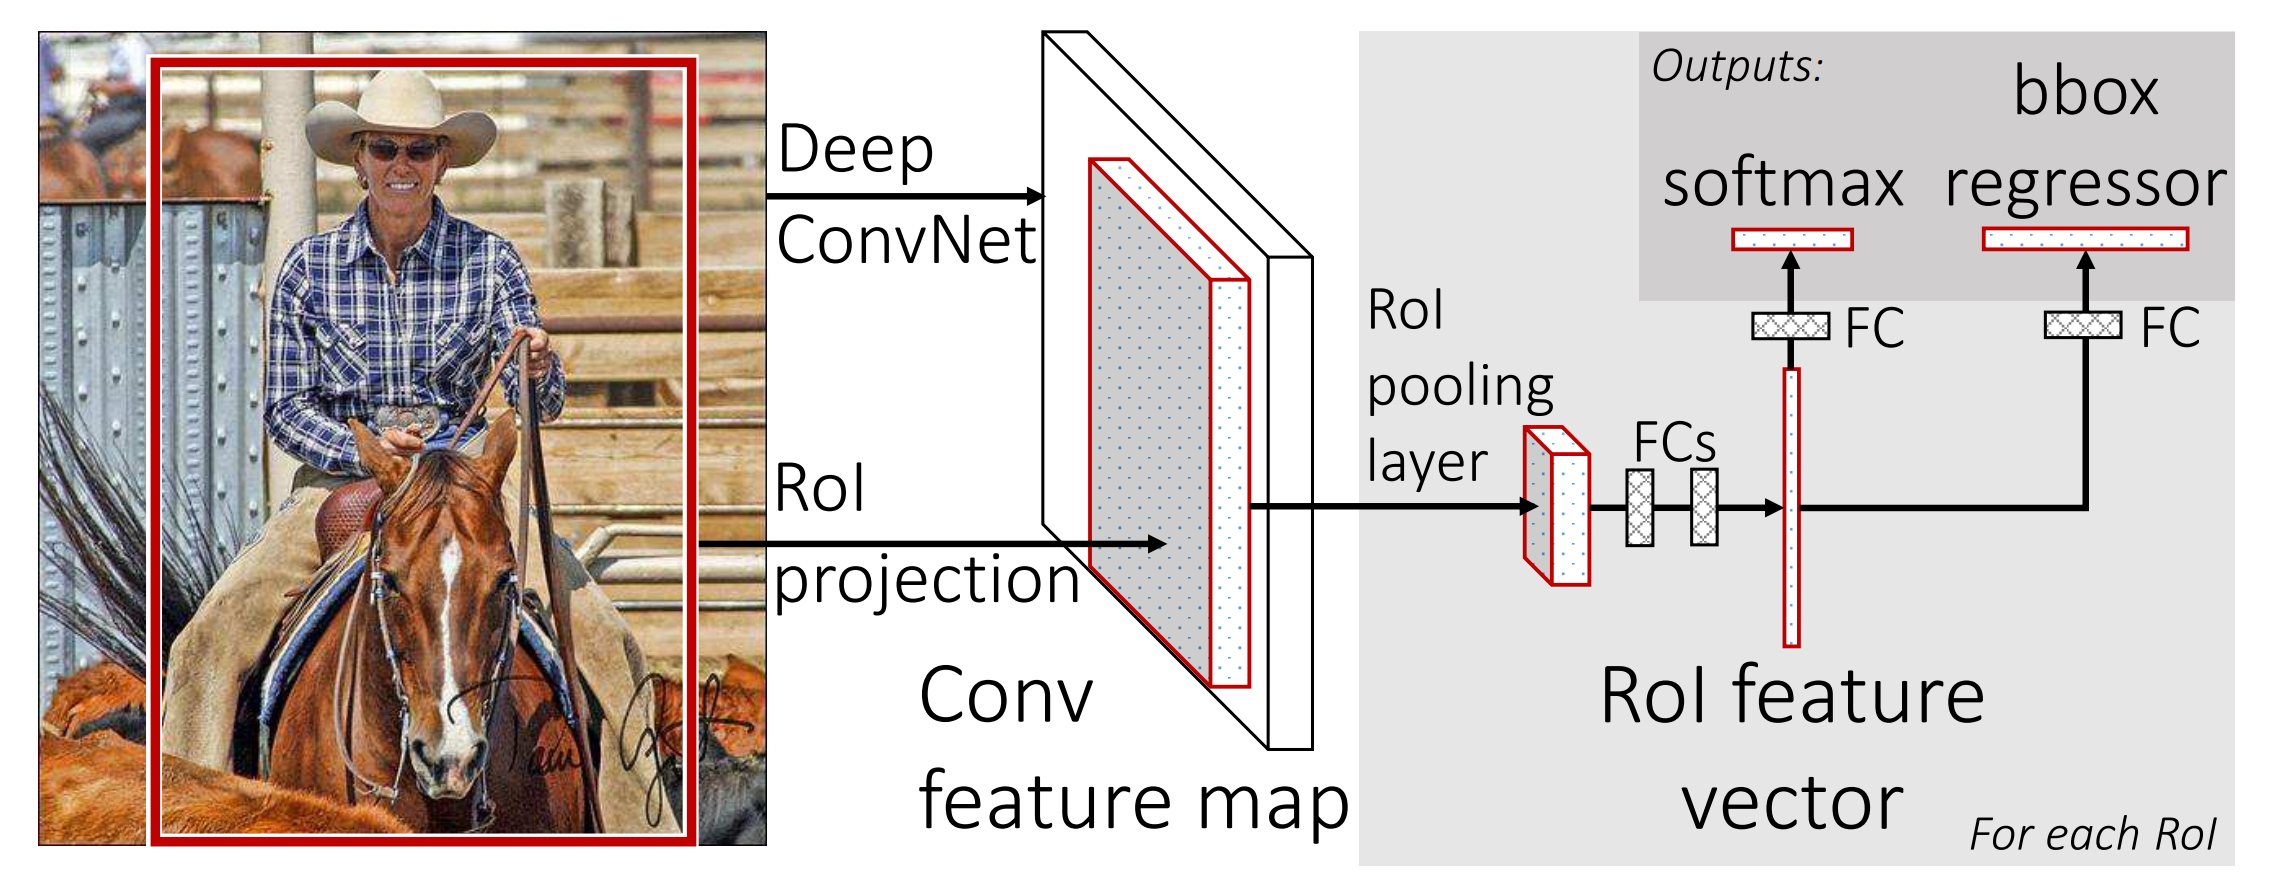
\includegraphics[width = 0.9\textwidth]{fastr.png}
    \caption{Fast R-CNN算法框架}
    \label{fastr}
\end{figure}

2016 年 Ren 等人针对候选区域提取速度的问题,提出了 Faster R-CNN 算法
\cite{ren2015faster},Faster R-CNN 算法框架如图\ref{fasterr}所示。

\begin{figure}[htbp]
    \centering
    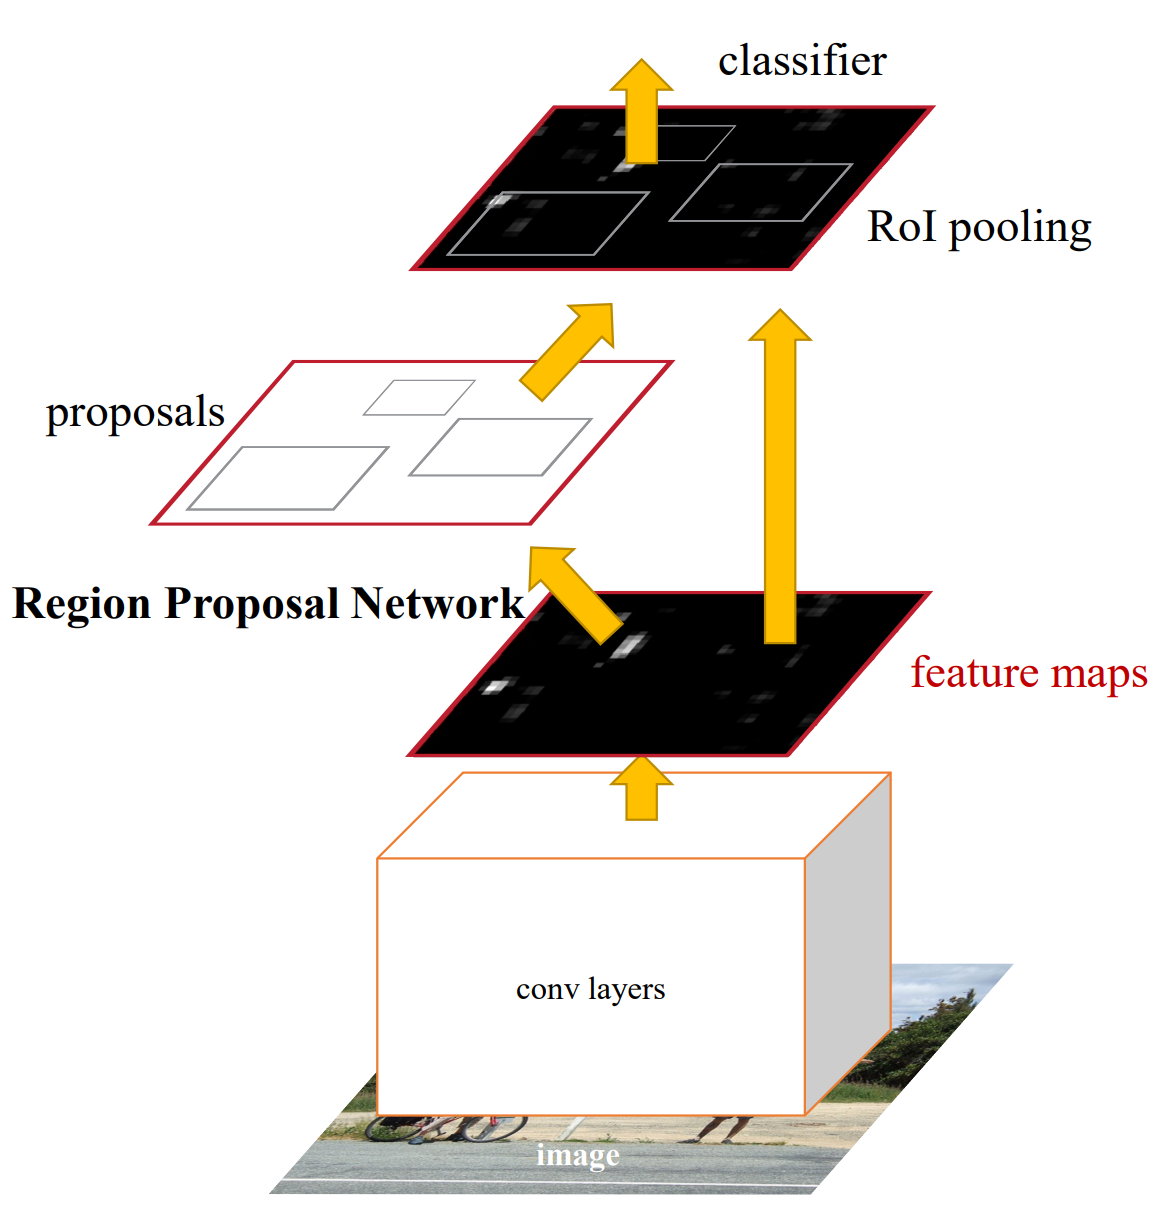
\includegraphics[width = 0.9\textwidth]{fasterr.png}
    \caption{Faster R-CNN算法框架}
    \label{fasterr}
\end{figure}

Faster R-CNN 创新地使用 Region
Proposal Network(RPN)网络替代 Selective Search 算法,由于 RPN 与检测网络
共享全图的卷积特征并且具有一组公共的卷积层,因此可以实现 end-to-end 的训
练网络。整个算法的实现过程为:

(1)输入整张图像到 VGG-16 进行特征提取。

(2)使用 RPN 生成 proposals。RPN 是一个全卷积网络,通过 n*n 的滑动窗口在特征
图上滑动,以窗口为中心在特征图的每个位置上用 9 种(三种尺度,三种长宽比)
anchor 生成 proposals,然后对每个 proposal 进行判断是否为背景和初步的回归。

(3)将 RPN 的输出再送入到 Fast R-CNN,通过 ROI pooling 输出固定大小 feature
map 后做更精细的分类和检测框的位置修正。

NIPS2015 版本的 Faster R-CNN 使
用的检测框架是 RPN+Fast R-CNN 网络进行目标检测,整体流程跟 Fast R-CNN一样,在 PASCAL VOC 2007 和 2012 数据集上测试 mAP 达到了 73.2%相比于
Fast R-CNN 速度提升了 10 倍。
该算法的局限在于以 ROI 池化层为界,前面的子网络用于特征提取,后面
的子网络用于目标检测,并且在对候选框进行分类和回归时需要分别输入到全卷
积网络进行计算,计算量大,达不到实时检测的目的并且对于小目标的检测效果
比较差。

在 Faster R-CNN 之后,基于候选框的目标检测算法仍有很多进展,目前具
有代表性的为 R-FCN\cite{dai2016r}和 Mask R-CNN\cite{he2017mask}。Faster R-CNN 虽然实现了网络端到
端的训练,但是整个网络以 ROI 池化层为界前面是共享全卷机网络,但是在 ROI
池化层后为 FC 层对每个 ROI 进行分类和回归,不是共享计算,因此导致整个算
法的运行速度慢。针对算法所使用的网络来说,backbone 如果卷积层数越深,所
获得的语义特征越多,越有利于分类任务的完成,但网络层数加深的同时会丢失
目标的位置信息,因此会导致网络对目标定位能力下降。由于目标检测网络不仅
需要对图片中的目标进行分类还要输出目标的位置,针对 ResNet、GoogLeNet
等深度网络提出分类网络 translation invariance 和检测网络 translation variance 平
衡问题,R-FCN 提出了 position-sensitive score mAP。R-FCN 使用 ResNet-101(去
掉最后一层 FC 层)作为 backbone,conv4 的输出作为 RPN 输入获得 ROI,网络
最后输出的 feature map 用来获得 position-sensitive score mAP 分别进行回归和分
类,在不损失精度的情况下运行速度比 Faster R-CNN 快 2.5 倍以上。算法框架如图\ref{rfcn}所示。

\begin{figure}[htbp]
    \centering
    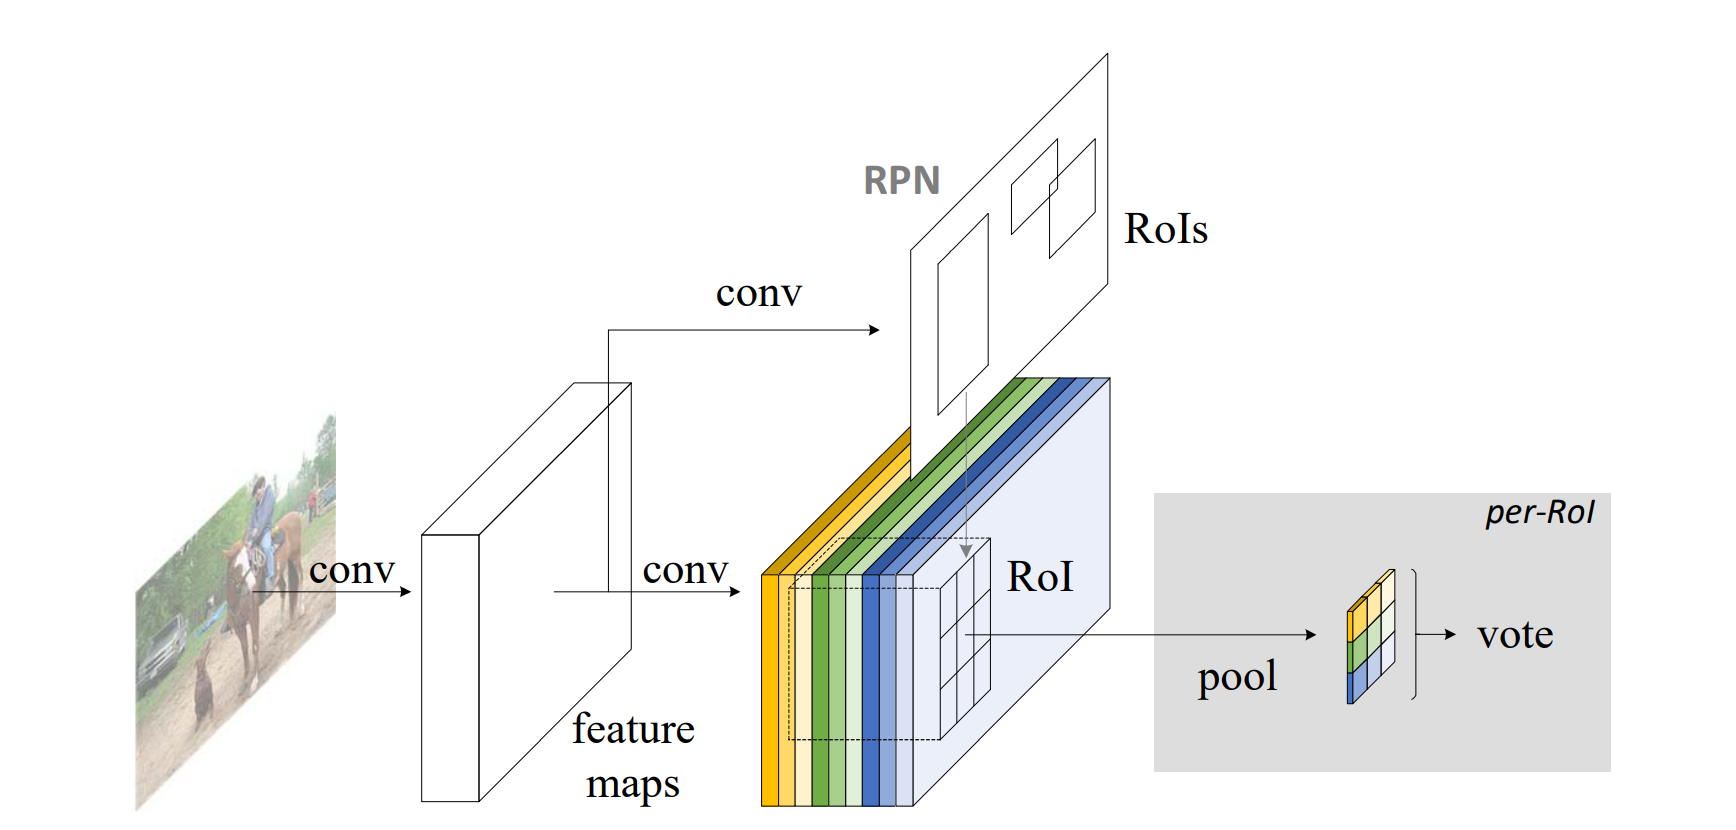
\includegraphics[width = 0.9\textwidth]{rfcn.png}
    \caption{R-FCN算法框架}
    \label{rfcn}
\end{figure}

Mask R-CNN 是以 Faster R-CNN 为原型,增加了一个 mask 分支
用于实例分割任务,此网络最大的创新点在于 ROI Align 的提出,解决了目标映
射到 feature map 上可能会出现坐标不是整数问题。ROI pooling 层需要输出固定
大小的 feature map 而进行等比例缩放过程中引入了量化误差,虽然量化只是去
掉了小数部分,但是映射到原图上误差会成倍的增长,从而严重影响网络的定位
准确性。在 ROI Align 中提出了双线性插值填补非整数位置的像素,使用 max 或
average pooling 汇总结果,整个过程没有使用量化,从而获得更准确的像素信息,
进一步提高了检测的精度,算法框架如图\ref{maskr}所示。

\begin{figure}[htbp]
    \centering
    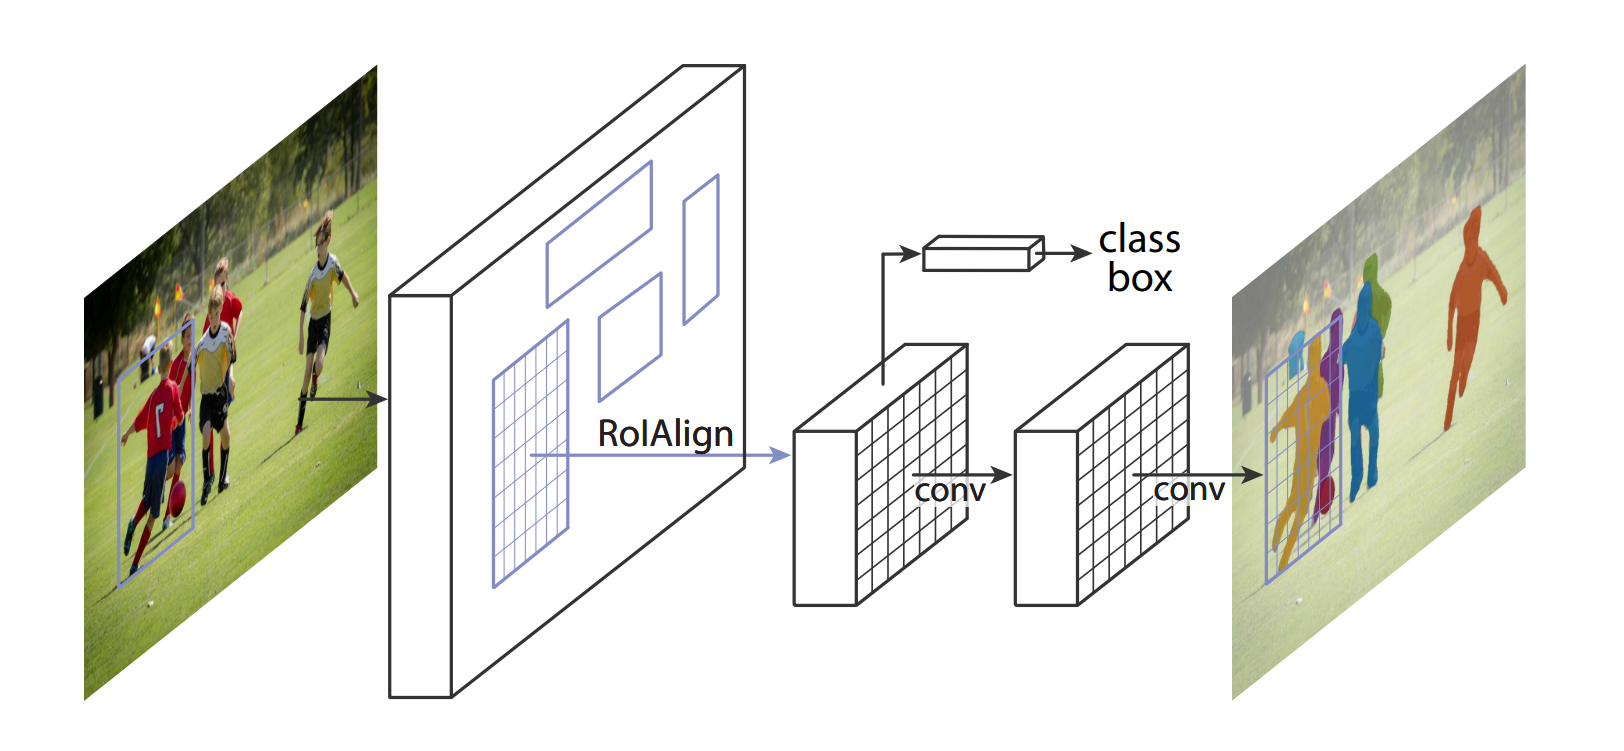
\includegraphics[width = 0.9\textwidth]{maskr.png}
    \caption{Mask R-CNN算法框架}
    \label{maskr}
\end{figure}

\subsection{基于深度学习的one-stage目标检测算法}
基于候选框的目标检测算法速度提升的关键是将目标检测问题转化为多区
域分类问题,充分利用目标在整个图片的上下文信息。对此,研究者们提出了一
种速度比基于候选框的目标检测算法快很多的基于回归的目标检测算法,基于回
归的目标检测算法没有候选框生成阶段,而是将图像上所有位置都视为潜在对象
去尝试对每个感兴趣的区域进行分类\cite{jiao2019survey,wu2020recent}。
2016 年 Redmon 等人提出的 YOLO(You Only Look Once)将目标检测看作
是回归问题\cite{redmon2016you},整个框架将目标分类和定位通过一个单一的网络完成,省略了候
选框生成步骤。YOLO 框架为图\ref{yk}所示,YOLO 直接在输出层回归 bounding box
的位置和所属类别,从而实现 one-stage。YOLO 的目标检测流程为:

\begin{figure}[htbp]
    \centering
    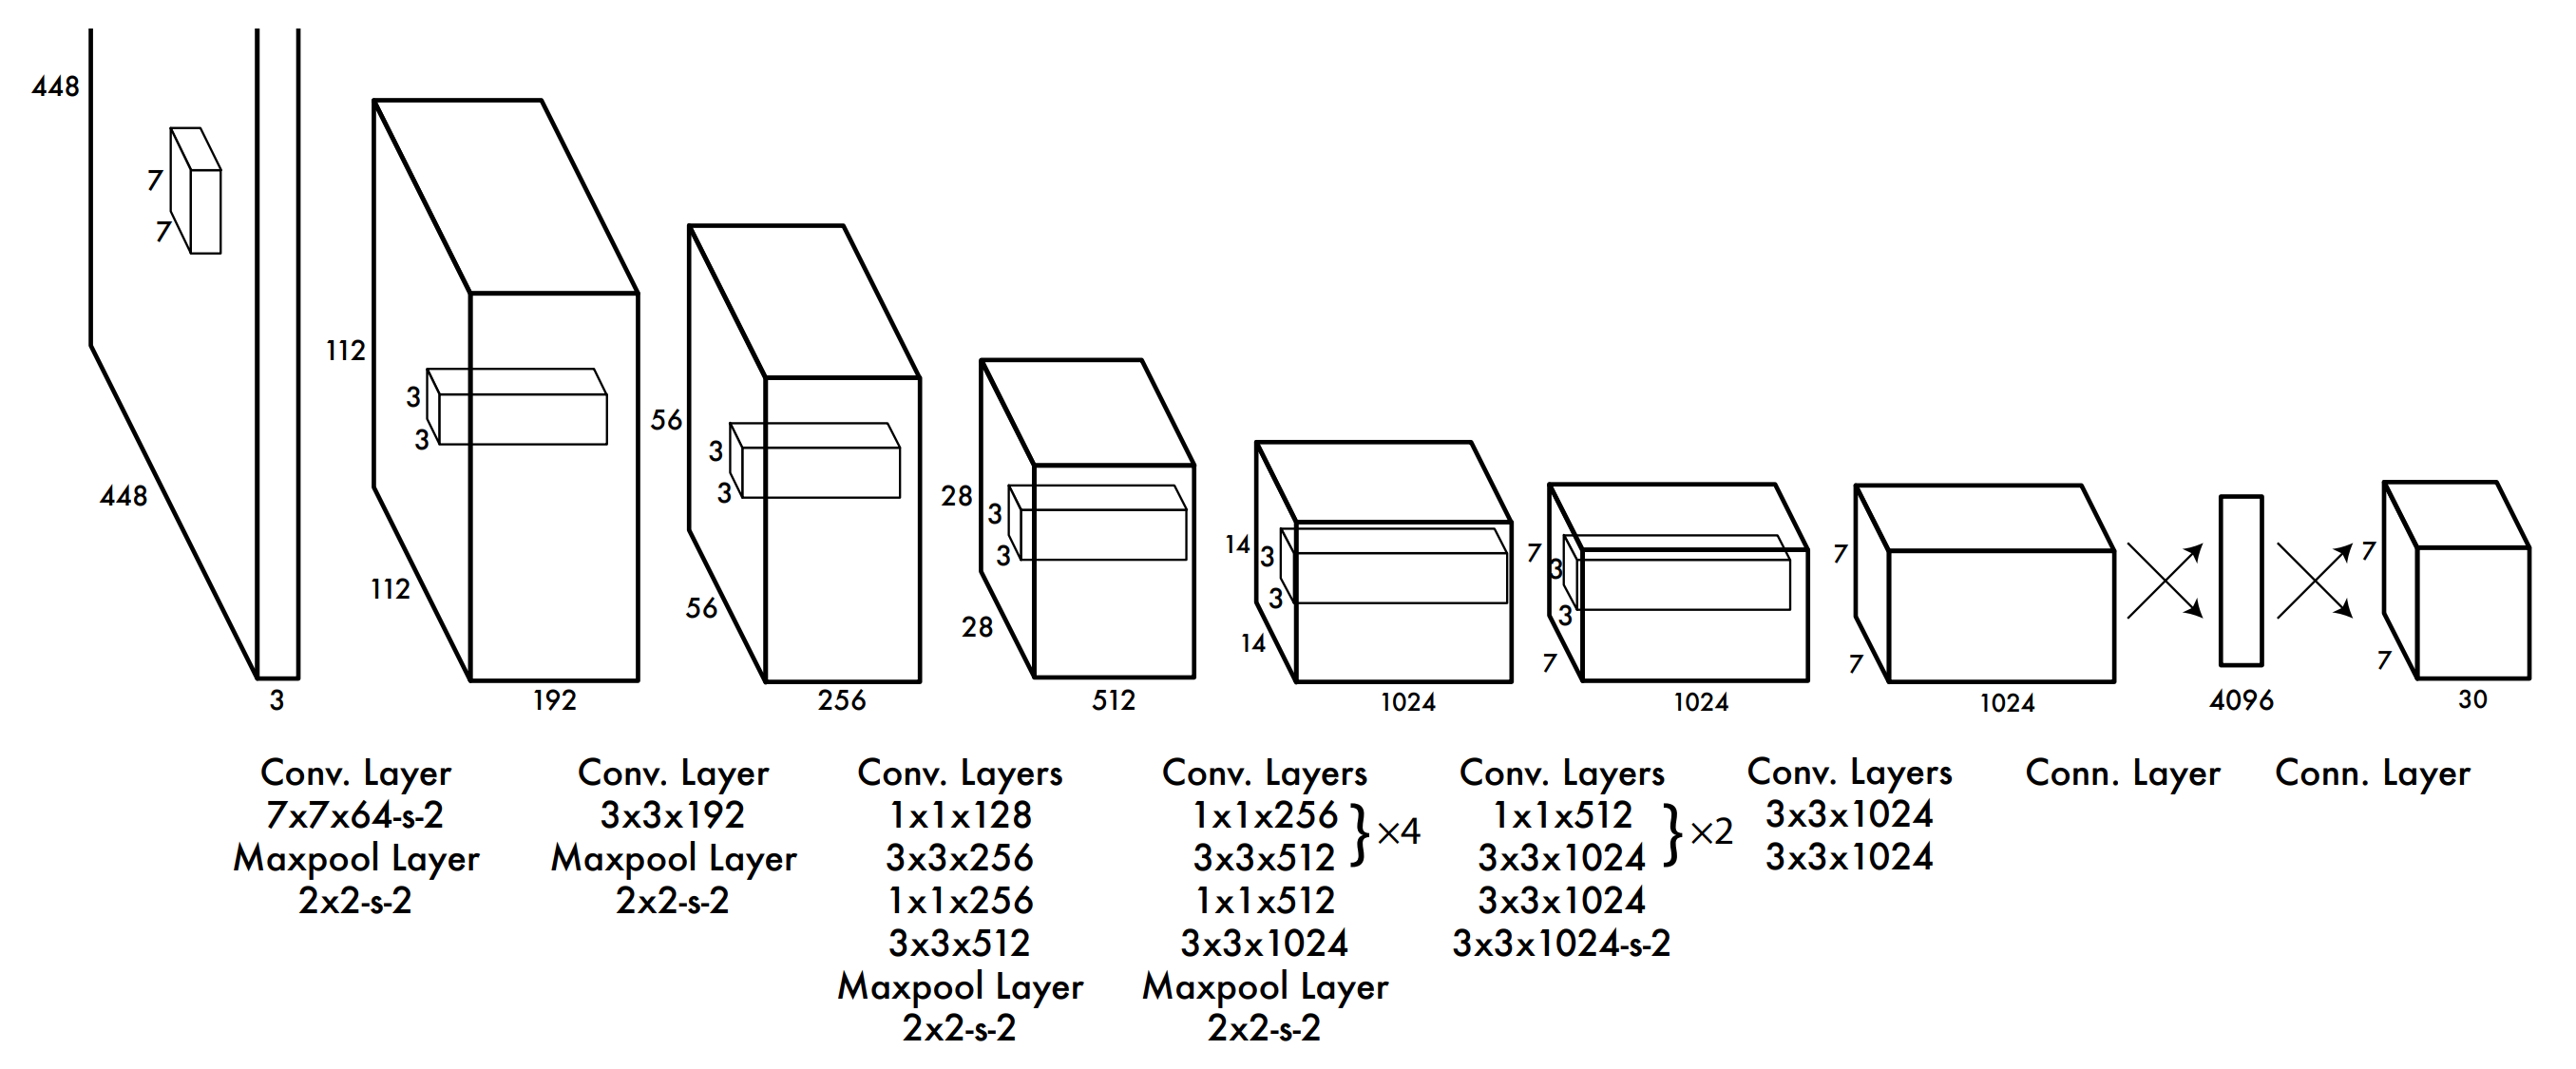
\includegraphics[width = 0.9\textwidth]{yolo框架.png}
    \caption{YOLO算法框架}
    \label{yk}
\end{figure}

(1)将输
入的图像划成 7*7 个网格;

(2)对每个网格预测两个 bounding boxes(每个
bounding box 包含五个参数(x,y,w,h,confidence)以及类别概率);

(3)对最后
输出的 7*7*2 个预测窗口设置阈值用 NMS 去掉可能性低的窗口。这样设计网络
在候选框处理过程中节省了时间,加快了网络的推理速度,经过测试 YOLO 可
以达到每秒 45FPS 的检测速度,能够达到实时性的要求。

YOLO 算法的局限性在于:

(1)要求输入图片的尺寸固定(448*448)

(2)
由于在每个网格上只能预测两个 bounding boxes,难以检测到小目标或目标比较
密集的情况,难以实现精准定位。

(3)检测不同大小的 bounding box 在损失函
数中的权重相同。总的来说虽然 YOLO 能够实现实时检测但是检测的精度却远
远不如 Faster R-CNN 等双阶段网络。

之后 YOLO 系列在保持检测速度的基础上对如何提升检测精度进行不断地
探索,提出了 YOLOv2\cite{redmon2017yolo9000}和 YOLOv3\cite{redmon2018yolov3}算法。YOLOv2 在 YOLO 的基础上进行
了多方面的改进:

(1)设计了新的分类网络(Darknet-19)作为 YOLOv2 的基
础网络,去掉了全连接层,使得网络输出的 feature map 分辨率增大,减少了计
算量的同时加快了检测的速度。

(2)引入了 Faster R-CNN 中的 anchor box 思想,
在每个 grid 设定 9 个 anchor 并且使用了 multiscale training,使得网络能够处理不
同尺寸输入的同时提高了网络的召回率和检测的精度。

(3)在每个卷积层使用
Batch Normalization,防止随着网络层数的加深导致的过拟合。YOLOv3 在
YOLOv2 的基础上借鉴了 FPN 思想,在 3 个不同大小的特征尺度上进行预测,
每个 grid 设置 3 个先验框,根据不同大小的特征图感受野不同来预测不同大小的
目标,每个候选框输出“位置偏移”,置信度以及分类结果。并且借鉴 residual
network 设计出网络层数更深功能更强大的 Darknet-53 作为基础网络,大大的提
高了检测的速度。损失函数使用 logistics 代替原来的 softmax 实现多标签分类,
适应更复杂的数据集。该算法在小目标上的精度提升比较明显,在中型和大尺度
目标的精度相比 YOLOv2 有所下降。

one-stage 算法另外的一个分支是 SSD 系列,在 2016 年 Liu W 等人提出的
SSD\cite{liu2016ssd}借鉴了 YOLO 的回归思想及 Faster R-CNN 的 anchor 机制,旨在高精度下
进行快速检测,使用多个尺度的特征图对不同大小的目标进行检测并最后将检测
结果进行合并,使得整个网络既能够像 YOLO 算法一样保持速度优势的同时使
网络预测到的先验框能够达到 Faster R-CNN 的准确度。从 YOLO 和 SSD 的结构
图可以看出,SSD 将不同层输出的不同大小的 feature map 都用来进行目标位置
和类别的训练和预测,从而达到多尺度检测的目的,而 YOLO 只是在最后一层
做目标位置和类别的训练和预测,由于最后一层的 feature map 比较小,对应的
anchor 到原图上的区域会较大,导致小目标的检测效果下降。SSD 与 YOLO 检
测模块的区别是造成 SSD 在小目标精度比 YOLO 提升明显的主要原因。算法框
架如图\ref{ssd}所示。

\begin{figure}[htbp]
    \centering
    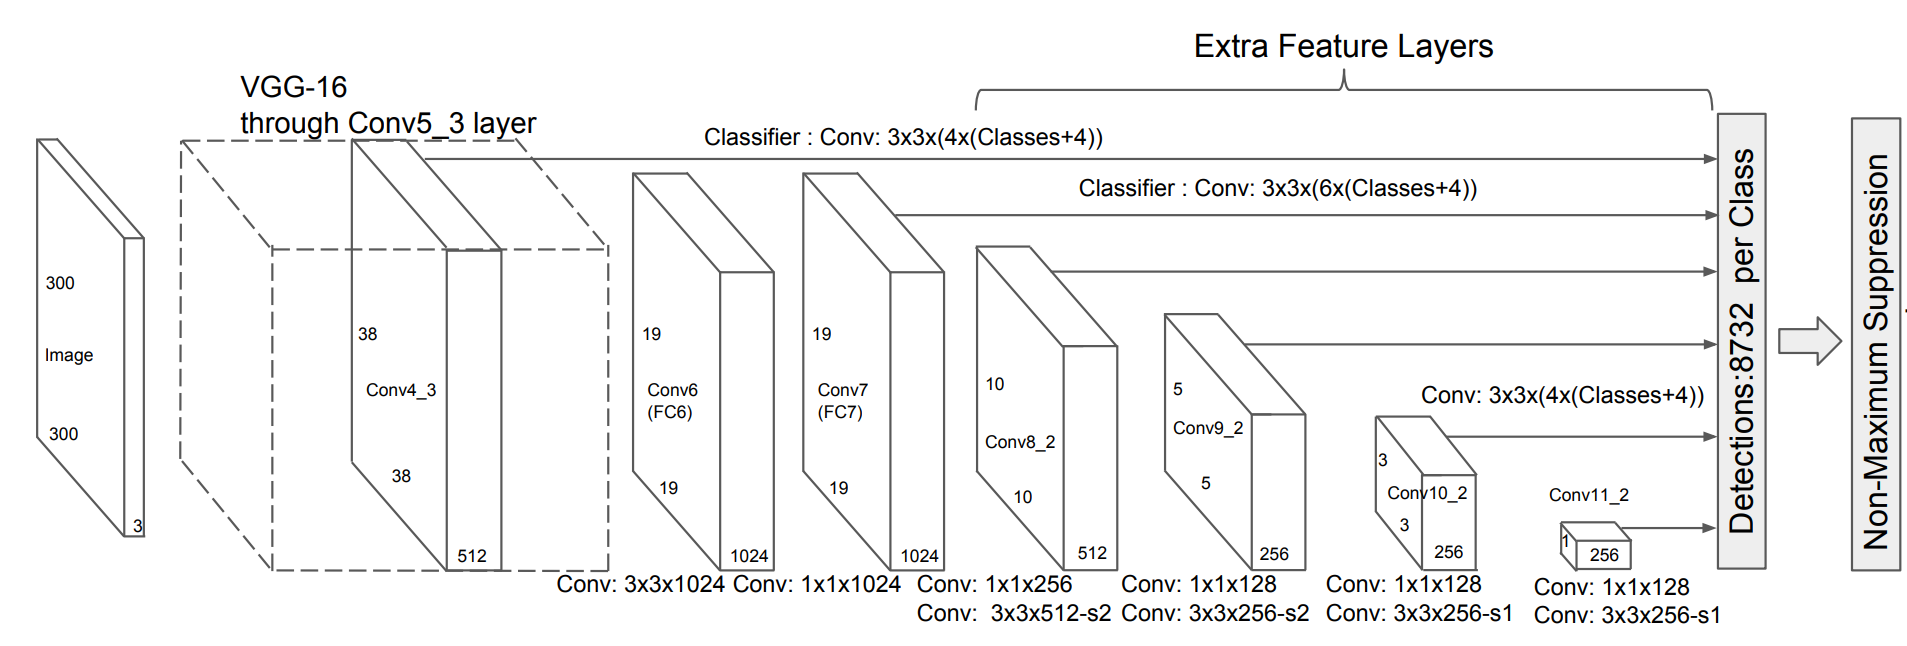
\includegraphics[width = 0.9\textwidth]{ssd.png}
    \caption{SSD算法框架}
    \label{ssd}
\end{figure}

最近几年基于 SSD 基础上的改进版本也很多,主要有 DSSD\cite{fu2017dssd}、
DSOD\cite{shen2017dsod}、FSSD\cite{li2017fssd}等。DSSD 主要针对 SSD 算法的浅层 feature map 语义信息不
够充分导致对小目标不够鲁棒的问题,提出了用 ResNet-101 和 Deconvolution 模
型,使用反卷积将特征图进行上采样与原始特征图进行融合,skip 连接使浅层
feature map 具有更好的表征能力。以前的目标检测算法都是先在开源的数据集上
进行预训练,然后再进行微调(fine-tuning),虽然 fine-tuning 可以加速获得最终模
型,但是获得的模型结构灵活性差,计算量也大。针对以上问题 DSOD 算法提
出一种不需要预训练模型的目标检测算法,网络可以从零开始训练,并且效果可
以和 fine-tuning 的模型媲美。DSOD 可以看作是 SSD+DenseNet 的结合,减少了
参数量。

\subsection{红外图像目标检测研究现状}
近年来随着红外成像技术的发展,红外目标检测任务也成为了重点研究的问
题之一。但红外图像往往会存在着对比度低、缺少目标纹理信息、信噪比低等特
点,使得红外目标检测任务增加了难度。因此如何攻克因红外图像特性带来的技
术难点,是未来红外目标检测的发展方向。
目前红外目标检测方法主要分为以下几种类别:基于目标的先验知识进行目
标检测、使用模板对目标进行匹配、基于机器学习方法进行目标检测等。

基于目标的先验知识进行目标检测的方法主要是用于红外场景简单并且目
标与背景之间对比度比较高的情况。此类方法往往需要人为的去建立一个数据库
作为先验知识,后续根据检测目标的特征与数据库进行比对。此种方法不但复杂
并且一旦检测其他的目标或检测环境发生变化时,就需要从新获取先验知识,因
此此类方法灵活性差,没有适用性。

使用模板对目标进行匹配的红外目标检测方法是利用统计的方法从之前的
数据中得到模板,然后将红外探测器获取到的红外图像与模板进行相似性度量,
根据二者相似度,从而实现对红外图像中的目标进行定位以及类别的确定\cite{宋曦2010一种基于模板匹配的目标识别方法}。

1997 年,Maes 等人提出了最大互信息图像匹配方法,相比传统算法减少了计算
量,之后广泛应用于目标检测等多个领域\cite{maes1997multimodality}。1999 年,Studholme C 等人考虑重
叠统计量作为重要因素,提出将梯度引入互信息中解决联合熵的不足,并针对互
信息不能提供有用的对齐措施问题将互信息进行归一化处理,实验结果显示能够
实现对目标的快速检测\cite{studholme1999overlap}。之后几年,Russakoff 等人提出互信息作为图片相似
性度量,没有考虑每个像素之间的关系,缺少空间信息。因此将空间信息引入到
互信息中进行扩展,提出了新的相似性度量方法-区域互信息\cite{russakoff2004image}。2005 年,顾静
良等人针对复杂背景下获得的红外图像具有大量的噪声并且存在弱小目标的情
况下,提出了一种适合红外弱小目标识别的相似性度量方法,并使用自适应模板
匹配方法来提高算法的稳定性\cite{顾静良2005基于自适应模板匹配的红外弱小目标检测}。2008 年,钟都都等人提出了一种改进的基于
模板匹配的跟踪算法,改良传统的模板匹配方法,用 SUSAN 算子提取目标的角
点特征,将特征信息和灰度信息进行加权融合来提取模板,所提出的算法用于红
外跟踪系统不仅能保证实时性,还具有稳定性和抗漂移能力\cite{钟都都2008用于红外目标跟踪的模板匹配改进算法}。虽然使用模板对
目标进行匹配的方法实现起来比较简单,但对模板的选择有很高的要求,同时如
果模板比较简单难以适用于复杂场景,如果将模板进行改进又会增加工作量,难
以适应各种场合以及目标的需要。因此目前该方法已逐渐被基于机器学习的方法
所替代,除了偶尔应用在简单场景下的工程项目外,几乎很少有应用。
基于机器学习的红外目标检测方法主要分为两类:一类是通过手工提取特征
对红外图像中感兴趣的区域(ROIs)进行提取最后使用分类器进行分类。主要分
为区域选择、特征提取和分类器分类三个步骤。之后还有基于目标特性进行 ROIs
区域搜索、阈值分割等方法。在深度学习出现之前,基于机器学习的红外目标
检测算法因其较强的鲁棒性,成为红外目标检测使用的主流算法。但由于该类算
法存在大量的计算冗余并且因为红外图像本身存在大量的噪声等特性,使得该算
法用于红外目标检测上的效果并不好。随着近年来深度学习的发展,卷积神经网
络强大的特征提取能力以及大数据处理能力,在可见光目标检测上取得了巨大的
成功。近几年也陆续出现了使用深度学习算法进行红外目标检测的研究。Aparna
Akula 等人为了开发一种隐私保护系统来实现自动识别人的行为,通过自建红外
数据集,并针对数据集设计目标检测网络,检测精度达到 87.44%,验证了卷积
神经网络用于红外目标检测的可行性\cite{akula2018deep}。许来祥等人结合红外图像的特点,提出了一种基于 ZFNet 改进的目标检测网络,在 ZFNet 基础上加空间变换网络提高
鲁棒性,并深入讨论 Dropout 层设置参数不同带来的影响\cite{许来祥2020基于改进}。虽然目前基于深度
学习的红外目标检测识别的研究并不多,但之后随着开源红外数据集的增多,相
关的研究会越来越多。

\section{本文主要研究内容}
本文主要针对红外图像无人机目标检测任务存在的问题进行研究,在课题研究过程中,主要分析并研究了以下几个方面的问题:

(1)红外无人机数据匮乏

目前开源的红外数据比较少,而基于深度学习的目标检测网络需要有充足的
数据支撑,因此本文的研究内容包括了红外无人机目标数据集的标注和制作。

(2)红外图像的检测特点和难点

由于红外图像在获取的过程中主要受到红外探测器和环境噪声的影响以及
红外辐射原理所造成的红外图像质量差、信噪比低等不利于检测的缺点。因此在
网络输入图像之前对红外图像进行预处理提高图像信噪比、增大图像包含的信息量也是重点研究的内容。

(3)待测无人机目标的尺度变化

本文的任务是红外图像无人机目标检测,场景的特点是小目标的出现频率较高,因此算法对较小尺寸目标的检测能力也是本文的研究内容。

(4)无人机目标检测的定位问题

在 YOLOv5 中使用IoU作为损失函数,有可能产生定位不准的问题,因此本文重点研究了对YOLOv5网络目标框定位损失函数的改进。

(5)检测算法的嵌入式实现以及实时推理

在某些特殊应用场景中难以满足较高的计算能力,如在嵌入式设备上使用,
无法保证在速度较快的情况下实现高精度检测,这种时候就需要设计出适用于特
定任务下的轻量级实时目标检测网络,也是本课题重点研究的问题。

\section{本文组织结构}
本文以红外目标检测算法所存在的问题展开研究,研究了红外无人机检测并实现嵌入式应用。本文分为四个章节,每
个章节的主要内容如下:

第一章为绪论。首先介绍了基于深度学习的红外目标检测算法的研究背景和
意义,然后针对当前主流的目标检测算法的国内外研究发展现状做了发展脉络介
绍,介绍了红外目标检测算法在传统方向和深度学习方向的相关研究工作,最后
介绍了本文具体的研究内容和组织结构。

第二章介绍了红外目标检测相关理论和工作基础。首先介绍了卷积神经网络
的主要组成结构以及目标检测的评价指标,接着对红外图像如何获得的过程进行
了简单的介绍,最后介绍了红外图像的主要特征。

第三章主要介绍了建立红外无人机图像数据集的过程,研究了目前主流的图像预处理方法,并进行了测试,用以提高整
个图像的信息量,并提出了两种新的红外数据增强算法,并将该算法在数据集上
进行了测试和结果分析,此外还对YOLOv5网络的目标框定位损失函数进行了改进,并对改进后的算法进行了实验和分析。

第四章实现红外无人机检测的轻量化和实时嵌入式应用。由于实际项目需要完成对无
人机的实时检测,因此本文重点研究了算法的轻量化和嵌入式部署,将第三章中研究的较高精度的红外无人机检测算法通过轻量化方法实现精度和速度的平衡,然后将得到的新算法部署在嵌入式设备上,进行更加贴近红外无人机检测应用场景的功能测试,基本可以达到实时推理,验证本文研究算法的适用性。

